%% CIShell Specification
%%
%

\documentclass[pdftex,11pt,letterpaper]{report}
\usepackage[top=1in, left=1in, right=1in, bottom=1in]{geometry}
\usepackage[pdftex]{graphicx}
\DeclareGraphicsExtensions{.pdf,.png,.jpg,.mps,.eps}
\usepackage[pdftex]{hyperref}
\usepackage{color}

\hypersetup{
    pdftitle={Cyberinfrastructure Shell (CIShell) Core Specification 1.0},    %
    title pdfsubject={Cyberinfrastructure Shell (CIShell) Core Specification
    1.0}, 
    pdfauthor={}, 
    pdfnewwindow=true,      % links in new window
}

\usepackage{../mystyle}

\title{Cyberinfrastructure Shell (CIShell) \\
Core Specification \\
1.0 \\
\textbf{DRAFT}}
% \author{} % Will fill in later 
% \date{} % ditto

\input{./tex/api.tex}
\packagesheader{}

\begin{document}

\maketitle{}
\tableofcontents{}

\chapter{Introduction}

The Cyberinfrastructure Shell (CIShell) is an open source, community-driven
platform for the integration and utilization of datasets, algorithms, tools, and
computing resources. It is built specifically to enable (1) algorithm developers
to write and disseminate their algorithms in their favorite programming language
while retaining their intellectual rights after distribution; (2) data holders to
easily disseminate their data for use by others; (3) application developers to
design applications from custom sets of algorithms and datasets that interoperate
seamlessly; and ultimately (4) end-users to use existing datasets and algorithms
effectively.

\section{CIShell Platform Overview}

The CIShell Platform consists of Java interface definitions of algorithms, data,
services for algorithm developers, and services for application developers. Much
of the platform uses metadata and is fully defined.

%The next version should have this section.
%\section{What is New}

%This is the first release of the CIShell Platform Specification. Future
%versions will strive for backwards compatibility.

\section{Reader Level}

This specification is written for the following audiences:
\begin{itemize}
  \item Java algorithm developers
  \item Non-Java algorithm developers
  \item Framework and system service developers (system developers)
  \item Application developers building on CIShell
\end{itemize}

The CIShell Specifications assume that the reader has at least one year of
practical experience in writing Java programs. CIShell is built to run on the
OSGi Service Platform Release 4\footnote{http://www.osgi.org/Release4/Download}
and thus a working knowledge of OSGi is expected. OSGi (and thus CIShell) is highly dynamic and must be taken into consideration
when developing anything on CIShell.

Non-Java algorithm developers may not need to know any Java and should be mainly
concerned with the metadata definitions for algorithms and data. They may also
need to be aware of OSGi and the other services CIShell provides, but more than
likely will not directly interact with them.

\section{Conventions and Terms}

In this specification, algorithms are referred to in three different contexts. An
abstract algorithm, is the pure idea of the algorithm with no actual source code.
It is a series of steps sometimes put into psuedo-code and often published in
academic journals. An \class{Algorithm} with a capital A refers to the Java class
called Algorithm. And finally, an algorithm with a lowercase A refers to the
bundle of code and metadata that encompasses an algorithm written to work with
the CIShell Platform. This includes the implementation of
\class{AlgorithmFactory} and \class{Algorithm}, and the metadata, files, and
other code that go into an OSGi bundle.

All other conventions and terms are exactly the same as from OSGi's Core
Specification, section 1.4.

\section{Version Information}

This is the first release of the CIShell Platform Specification. All packages are
at 1.0 for this release. Subsequent releases may increase the version number of
specific packages if changes have been made.

\begin{table}[h!]
\begin{tabular}{l l l}
\textbf{Item} & \textbf{Package} & \textbf{Version} \\
Framework Specification & org.cishell.framework & Version 1.0 \\
Algorithm Specification & org.cishell.framework.algorithm & Version 1.0 \\
Data Specification & org.cishell.framework.data & Version 1.0 \\
Data Conversion Service Specification & org.cishell.service.conversion &
Version 1.0 \\
GUI Builder Service Specification & org.cishell.service.guibuilder & Version
1.0 \\
Data Manager Application Service Specification & org.cishell.app.datamanager &
Version 1.0 \\
Scheduler Application Service Specification & org.cishell.app.scheduler &
Version 1.0 \\
\end{tabular}
\caption{Packages and Versions}
\label{table:packageVersions}
\end{table}
%% Cyberinfrastructure Shell (CIShell) Core Specification
%%
%% Copyright 2006,2007,2008 Indiana University
%%
%% Licensed under the Apache License, Version 2.0 (the "License");
%% you may not use this file except in compliance with the License.
%% You may obtain a copy of the License at
%%
%%     http://www.apache.org/licenses/LICENSE-2.0
%%
%% Unless required by applicable law or agreed to in writing, software
%% distributed under the License is distributed on an "AS IS" BASIS,
%% WITHOUT WARRANTIES OR CONDITIONS OF ANY KIND, either express or implied.
%% See the License for the specific language governing permissions and
%% limitations under the License.
%%
%

\chapter{Framework API}

\section*{\textit{Version 1.0}}

\section{Introduction}

The \class{org.cishell.framework} package and subpackages define the core of
CIShell. The key components being algorithms, data, and CIShell service access.

\subsection{Entities}

\begin{itemize}
  \item \textit{AlgorithmFactory} - The service interface for algorithms.
  A factory class which creates an \class{Algorithm} for execution from input
  data.
  \item \textit{Algorithm} - The interface for the code execution part of the
  algorithm.
  \item \textit{AlgorithmProperty} - The interface which provides string
  constants for an algorithm's service metadata.
  \item \textit{ParameterMutator} - The interface an \class{AlgorithmFactory}
  extends to provide the ability to add, remove, or modify its input
  parameters specification (see section \ref{GUISpec}) before being transformed
  into a form for user input.
  \item \textit{DataValidator} - The interface an \class{AlgorithmFactory}
  extends to provide additional data validation in addition to the data format validation
  that an application should provide ahead of time.
  \item \textit{ProgressTrackable} - The interface an \class{Algorithm} extends
  to allow for more detailed monitoring and control of an \class{Algorithm}'s
  progress while executing.
  \item \textit{ProgressMonitor} - The interface for a class to be passed in to
  a \class{ProgressTrackable} \class{Algorithm} so that the \class{Algorithm}
  can be controlled and provide information on its progress while executing.
  \item \textit{Data} - The interface used to pass data (other than
  input parameters) and its metadata between algorithms.
  \item \textit{BasicData} - A simple implementation of the \class{Data}
  interface.
  \item \textit{DataProperty} - The interface which provides string constants
  for \class{Data} metadata.
  \item \textit{CIShellContext} - The interface for a class to be passed in to
  an \class{AlgorithmFactory} for use in gaining access to standard CIShell
  services.
  \item \textit{LocalCIShellContext} - A simple implementation of the
  \class{CIShellContext} interface which pulls CIShell services from the OSGi
  service registry.
\end{itemize}

\begin{figure}[htb!]
\centering
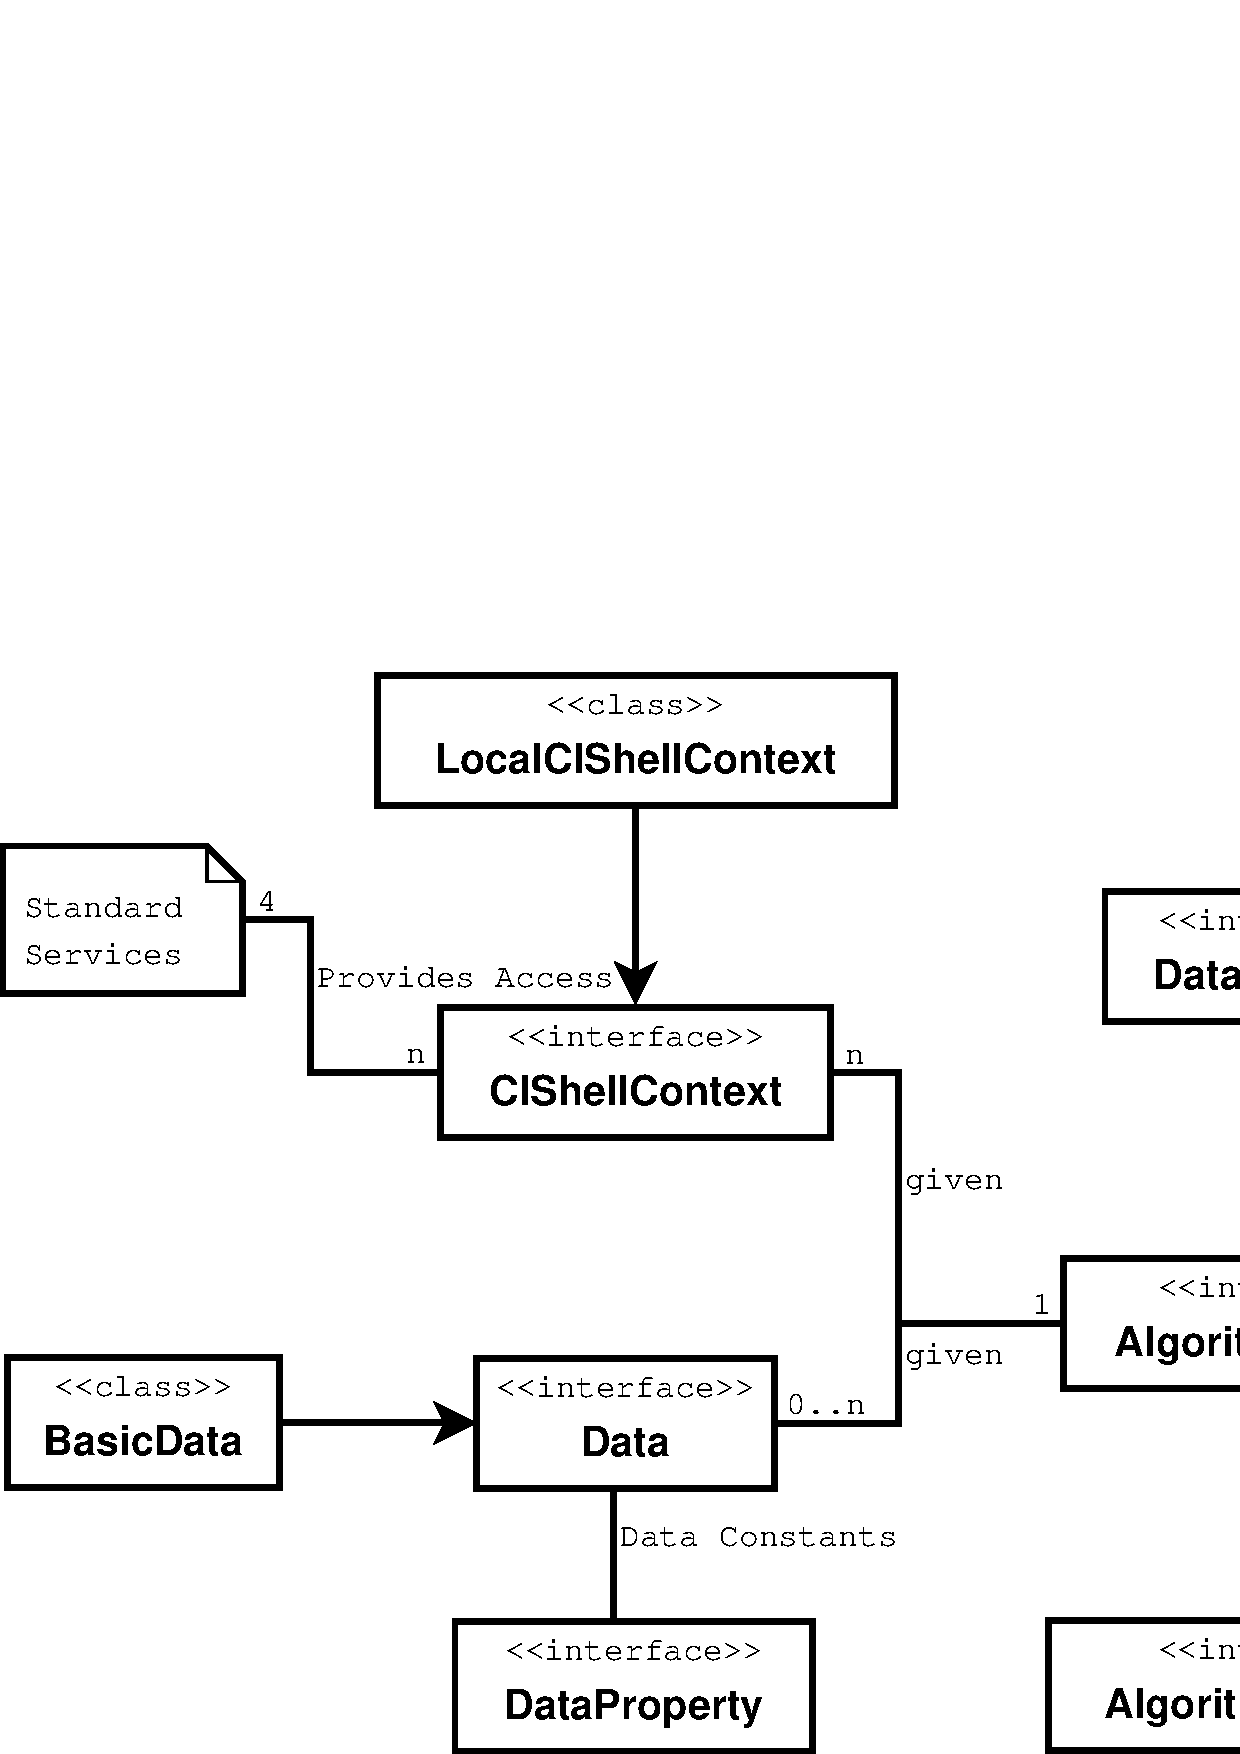
\includegraphics[width=150mm]{../img/cishellInteraction.pdf}
\caption{org.cishell.framework Class Diagram}
\label{fig:cishellInteraction}
\end{figure}

\subsection{Operations}

The algorithm developer should implement algorithms as described in this
specification. The system developer will provide the services required by CIShell
in OSGi's service registry. Application developers will provide everything else,
orchestrating the passing of information between algorithms.

%% Cyberinfrastructure Shell (CIShell) Core Specification
%%
%% Copyright 2006,2007,2008 Indiana University
%%
%% Licensed under the Apache License, Version 2.0 (the "License");
%% you may not use this file except in compliance with the License.
%% You may obtain a copy of the License at
%%
%%     http://www.apache.org/licenses/LICENSE-2.0
%%
%% Unless required by applicable law or agreed to in writing, software
%% distributed under the License is distributed on an "AS IS" BASIS,
%% WITHOUT WARRANTIES OR CONDITIONS OF ANY KIND, either express or implied.
%% See the License for the specific language governing permissions and
%% limitations under the License.
%%
%

\section{OSGi Dependencies}

CIShell is built to be run in a fully compliant OSGi Service Platform R4
implementation. In addition to the base OSGi implementation, several
optional OSGi services are required to be available in a fully compliant CIShell
implementation. Each additional required service is described in the OSGi
Service Platform Service Compendium
R4\footnote{http://www.osgi.org/Release4/Download}.

\subsection*{Required Services}
\begin{description}
  \item[Metatype Service] is described in OSGi section 105 ``Metatype Service
  Specification.'' This service is used by CIShell to find
  \class{MetaTypeProviders} for user interface specification, user-adjustable
  preferences, and input parameters. It also provides an XML format for
  automatically generating \class{MetaTypeProvider}s which the 
  \class{MetaTypeService} harvests for use.
  \item[Log Service] is described in OSGi section 101 ``Log Service 
  Specification.'' This service is used as a universal logging system for 
  algorithms and services. See chapter \ref{logService} for more details.   
  \item[Preferences Service] is described in OSGi section 106 ``Preferences
  Service Specification.'' This service is used as a universal preference
  storage system for algorithms and services. See chapter \ref{preferencesService} for
  more details.
  \item[Configuration Admin Service] is described in OSGi section 104
  ``Configuration Admin Service Specification.'' This service is used as a
  manager/provider of configuration information for bundles and services. It is 
  useful for meeting the User Adjustable Preferences (section
  \ref{userPrefsSpec}) requirements.
\end{description}

\subsection*{Recommended Services}
\begin{description}
  \item[Declarative Services] is described in OSGi section 112 ``Declarative
  Services Specification.'' This service can be used by CIShell algorithms to
  simplify algorithm service registration and for finding necessary auxilary services.
\end{description}

\section{Algorithm Specification}

\subsection*{\textit{Version 1.0}}

\subsection{Introduction}

The CIShell Platform has been specifically designed around the idea of the
algorithm. It is the central and most important concept. Algorithms are fully
defined and self-contained bits of execution. They can do many things from data
conversion, data analysis, and can even spawn whole outside programs if needs be.
Algorithms are very well defined black boxes in that what can come into and out
of the algorithm is specified in each algorithm's metadata. Other than that,
CIShell makes no attempt to understand the algorithm.

Figure \ref{fig:algExecWorkflow} shows the flow of information into and out of an
algorithm. Here an algorithm is passed zero or more pieces of data, any
user-entered parameters, and a CIShell context. The algorithm is then executed
and produces zero or more pieces of data.

\begin{figure}[htb!]
\centering
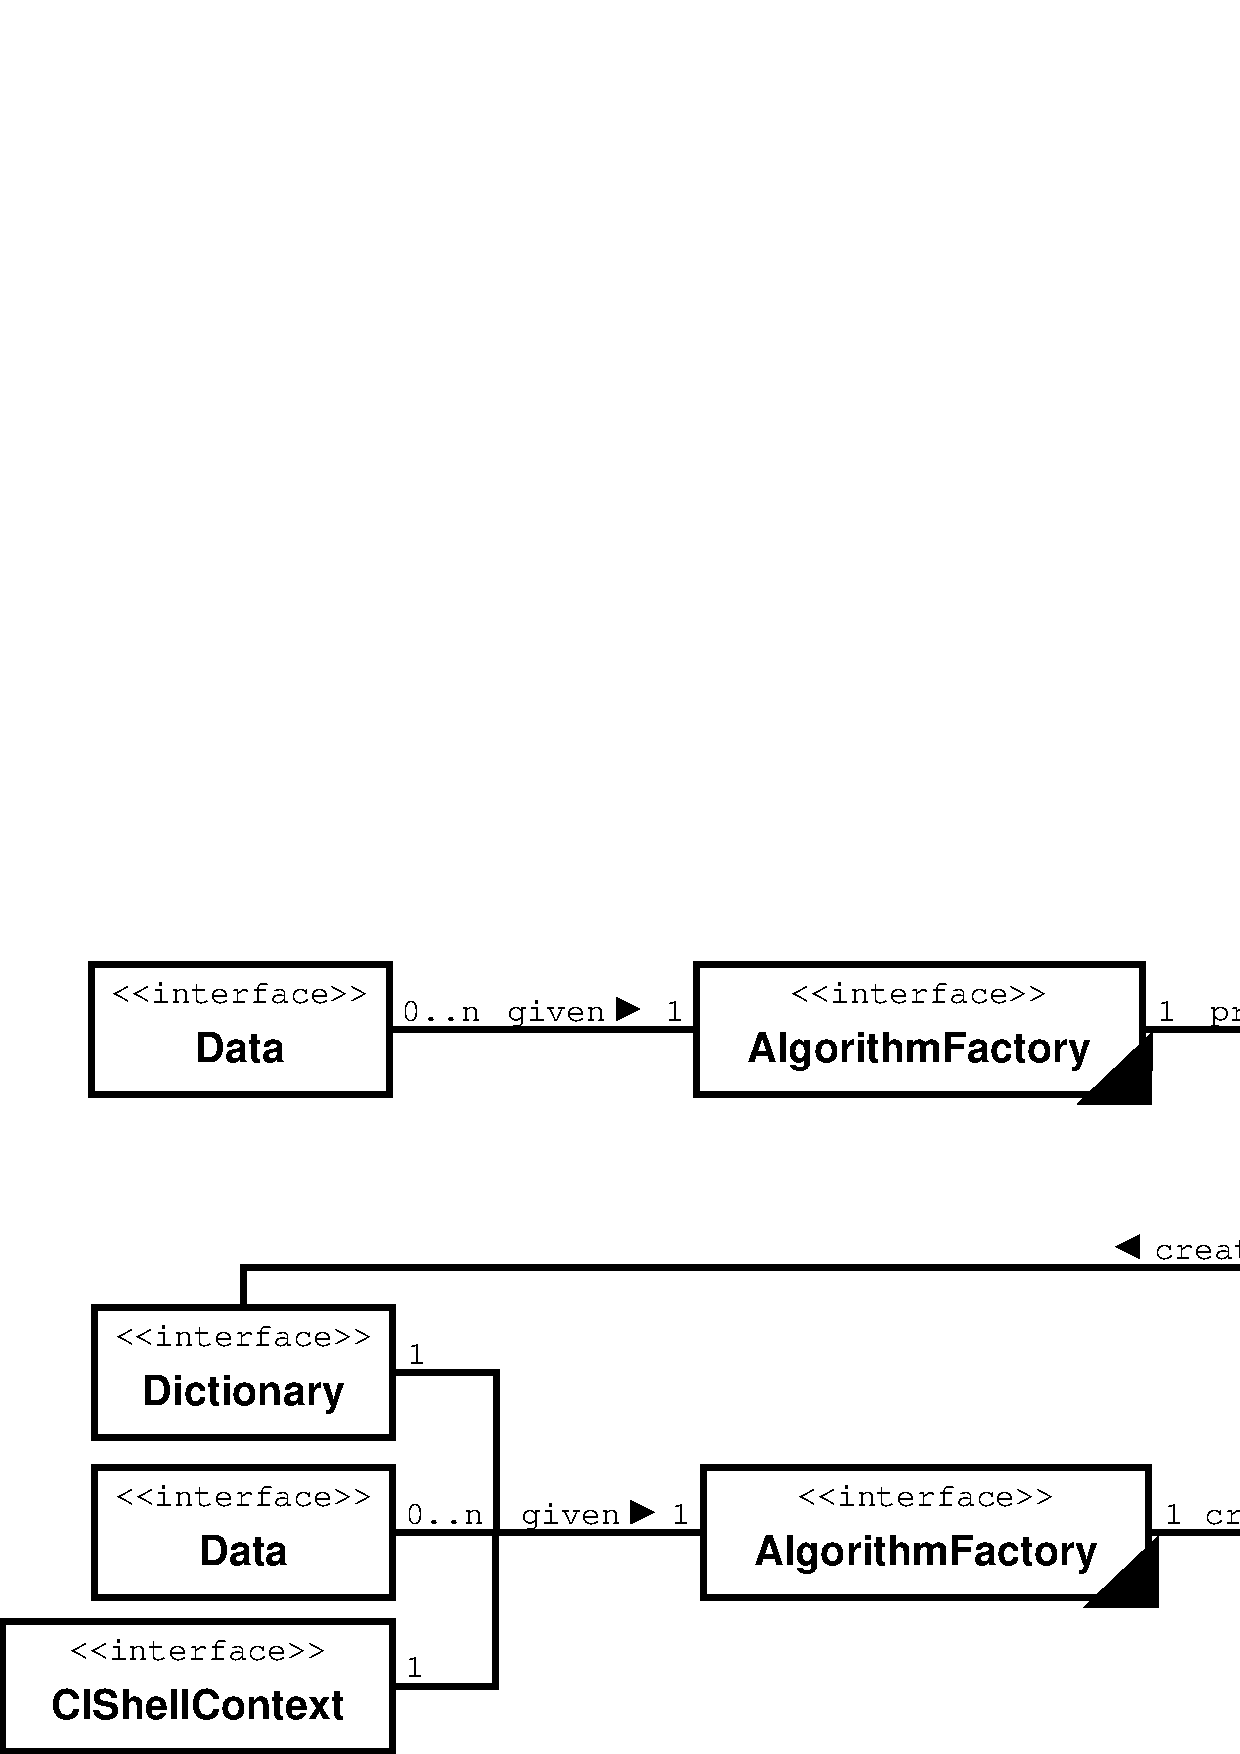
\includegraphics[width=150mm]{../img/algExecWorkflow.pdf}
\caption{Algorithm Execution Workflow}
\label{fig:algExecWorkflow}
\end{figure}

An algorithm defines its inputs in two ways. First, the input Data is defined
in the algorithm's service metadata. Second, the acceptable user-entered
parameters are defined in a MetaTypeProvider. This MetaTypeProvider defines the
types, value range, and textual description of the parameters needed. From this
information, a user interface (UI) can be created that asks a user for the
data.

\subsection{Standard Algorithm Properties}
\orgcishellframeworkalgorithm{}

\section{Algorithm Type Specifications}

\subsection*{\textit{Version 1.0}}

\label{algConstraints}

\subsection{Base Algorithm Constraints}

All conformant algorithms regardless of type, must adhere to the following
constraints:

\subsubsection*{Required:}
\begin{itemize}
  \item The algorithm must be a conformant \class{AlgorithmFactory}
  implementation and properly registered as a service.
  \item The algorithm's service metadata must contain a legal ``service.pid''.
\end{itemize}

\subsubsection*{Optional:}
\begin{itemize}
  \item The algorithm's service metadata should have ``remoteable=true'' if it
  meets the requirements of a remoteable algorithm.
  \item The algorithm's service metadata should have a ``label'' which is a
  short human-readable name for the algorithm.
  \item The algorithm's service metadata should have a ``description''
  describing what the algorithm does in more detail.
  \item As much of the informational metadata as possible should be
  provided. This includes ``authors'', ``implementors'', ``integrators'',
  ``documentation\_url'', ``reference'', ``reference\_url'', and ``written\_in''.
\end{itemize}

\subsection{Standard Algorithms}

Standard CIShell algorithms are the algorithms that most end-users will
encounter. A standard algorithm has the following constraints:

\subsubsection*{Required:}
\begin{itemize}
  \item The algorithm must be a conformant \class{AlgorithmFactory}
  implementation and properly registered as a service.
  \item The algorithm's service metadata must contain a legal ``service.pid''.
  \item The algorithm's service metadata must have a ``label'' which is a
  short human-readable name for the algorithm. This is typically used to label
  an algorithm for an end-user to see.
  \item The algorithm's service metadata must have a ``description''
  describing what the algorithm does in more detail.
  \item The algorithm's service metadata must have a ``menu\_path'' which is
  simultaneously a classification and a location on a GUI's menubar to place
  the algorithm in. See section \ref{algMetaData} for how to format a
  ``menu\_path''.
\end{itemize}

\subsubsection*{Optional:}
\begin{itemize}
  
  \item The algorithm's service metadata should have ``remoteable=true'' if it
  meets the requirements of a remoteable algorithm.
  \item The algorithm's service metadata should have ``parentage=default'' if
  it wishes to use the default \class{Data} parenting scheme described in
  section \ref{algMetaData}.
  \item The algorithm's service metadata does not need to have a ``type'' set.
  \item As much of the informational metadata as possible should be
  provided. This includes ``authors'', ``implementors'', ``integrators'',
  ``documentation\_url'', ``reference'', ``reference\_url'', and ``written\_in''.
\end{itemize}


\subsection{Converter Algorithms}
\label{converterAlg}

A converter algorithm is a custom type of CIShell algorithm for converting data
of one type to another. Converters are typically leveraged by the
\class{DataConversionService} and are not used directly by end-users. A converter
algorithm has the following constraints:

\subsubsection*{Required:}
\begin{itemize}
  \item The algorithm must be a conformant \class{AlgorithmFactory}
  implementation and properly registered as a service.
  \item The algorithm must take in a single \class{Data} item and convert the
  item producing a single \class{Data} item. This must be reflected in the
  algorithm's service metadata where ``in\_data'' and ``out\_data'' have only
  one format each.
  \item The algorithm's service metadata must contain a legal ``service.pid''.
  \item The algorithm's service metadata must have ``type=converter''.
  \item The algorithm's service metadata must have ``conversion=lossy'' if
  data is lost during conversion or ``conversion=lossless'' if not.
\end{itemize}

\subsubsection*{Optional:}
\begin{itemize}
  \item The algorithm's service metadata should have ``remoteable=true'' if it
  meets the requirements of a remoteable algorithm.
  \item The algorithm's service metadata should have a ``label'' which is a
  short human-readable name for the converter, usually with the common name of
  the input data format and output data format.
  \item The algorithm's service metadata should have a ``description''
  describing the conversion in more detail, especially what data may be lossed
  if ``conversion=lossy''.
  \item The algorithm's service metadata should have ``implementers'' filled
  in accordingly.  
\end{itemize}

\subsection{Validator Algorithms}

A validator algorithm is a custom type of CIShell algorithm which checks either
an incoming or outgoing file to be sure it is of the type specified. This is
necessary due to the fact that one cannot simply assume based on the file
extension what type of file format the data is in. Checking the contents of the
file is necessary, especially in the case of multiple file formats for the same
file extension (e.g., XML). This type of algorithm is important for reliably
bringing in outside data and saving out data from CIShell. A validator algorithm
has the following constraints:

\subsubsection*{Required:}
\begin{itemize}
  \item The algorithm must be a conformant \class{AlgorithmFactory}
  implementation and properly registered as a service.
  \item The algorithm must take in a single \class{Data} item and validate the
  item producing a single \class{Data} item (with the same data, but changed
  format) or \class{null} if the file being validated is not of the right
  type. This must be reflected in the algorithm's service metadata where
  ``in\_data'' and ``out\_data'' have only one format each with one containing
  a ``file:'' format and the other a ``file-ext:'' depending on the direction
  of validation.
  \item The algorithm must not alter the data. Its only purpose is to validate
  the proposed incoming or outgoing file.
  \item The algorithm's service metadata must contain a legal ``service.pid''.
  \item The algorithm's service metadata must have ``type=validator''.
  \item The algorithm's service metadata must have a ``label'' which is the
  common name of the data format being validated.
\end{itemize}

\subsubsection*{Optional:}
\begin{itemize}
  \item The algorithm's service metadata should have ``remoteable=true'' if it
  meets the requirements of a remoteable algorithm.
  \item The algorithm's service metadata should have ``implementers'' filled
  in accordingly.
\end{itemize}

%% Cyberinfrastructure Shell (CIShell) Core Specification
%%
%% Copyright 2006,2007,2008 Indiana University
%%
%% Licensed under the Apache License, Version 2.0 (the "License");
%% you may not use this file except in compliance with the License.
%% You may obtain a copy of the License at
%%
%%     http://www.apache.org/licenses/LICENSE-2.0
%%
%% Unless required by applicable law or agreed to in writing, software
%% distributed under the License is distributed on an "AS IS" BASIS,
%% WITHOUT WARRANTIES OR CONDITIONS OF ANY KIND, either express or implied.
%% See the License for the specific language governing permissions and
%% limitations under the License.
%%
%

\section{Data Specification}
\label{dataSpec}
\subsection*{\textit{Version 1.0}}
\subsection{Introduction}

Data to be operated on is passed around in \class{Data} objects which hold the
real data, the data's format, and the data's properties (metadata). The real
data can be any Java \class{Object}. The format is a string describing the 'format' of the
data, see next section. Finally, the properties help describe the data. The label
to give the data, the parent \class{Data} object from which it was derived from,
and a coarse data type can all be defined in the \class{Data}'s properties. See
the \class{DataProperty} interface definition for specific properties to use.

\subsection{Data Format Specification}

Data formats are used by algorithms specifying what \class{Data} items are
consumed/producted and \class{Data} objects must know what the format of its
contained real data is. This format is simply a string that says what the
format of the real data is. If the real data is a \class{java.io.File}, use a
MIME type\footnote{If no official mime type is available for a file format, a
made up one can be used, but must still conform to how mime types are
constructed, see RFCs 3023 (http://tools.ietf.org/html/rfc3023) and 4288
(http://tools.ietf.org/html/rfc4288).} prefixed by ``file:'', i.e.,
``file:\textit{mime/type}''. If the real data is a \class{java.io.File} known
only by file extension (only applicable for validator algorithms), use the format
``file-ext:\textit{file-extension}''. Otherwise, if the real data is a Java
\class{Object}, use the full Java class as a string, i.e., ``java.lang.String''
or ``my.package.SpecialClass''.

To specify that a single \class{Data} object contains one or more
sub-\class{Data} objects of a single format, prefix the type with a ``+''. For
zero or more, prefix the type with a ``*''. This corresponds to a \class{Data}
object that is wrapping multiple (zero or one or more depending on the prefix)
other \class{Data} objects of the associated format in a Java array
(\class{Data[]}) stored as its contained real data. This is useful for
algorithms that can work on a variable number of \class{Data} items.

\section{User Interface Specification}
\label{GUISpec}
\subsection*{\textit{Version 1.0}}
\subsection{Introduction}

For many algorithms, just looking at the data given isn't enough. Additional
parameters are often needed to know how to operate on a given piece of data. An
algorithm can define what parameters are needed by providing a
\class{MetaTypeProvider}. It defines the types, value range, and textual
description of the parameters needed. From this information, a user interface
(UI) can be created that asks a user for the data. The \class{MetaTypeProvider}
is not tied to any specific UI, so it can be reused depending on the context
(desktop application, web application, command line, etc.).

\class{MetaTypeProvider} is defined in the OSGi R4 Specification Service
Compendium as part of the Meta Type Service. \class{MetaTypeProvider}s can be
created in code or can be specified in an xml file (as defined in the
specification) and pulled out of the \class{MetaTypeService} service. A
\class{MetaTypeProvider} can be thought of as a collection of UIs. Each UI is
called an \class{ObjectClassDefinition}, which provides a UI name and
description and is a collection of parameters. Each parameter is an
\class{AttributeDefinition} which includes the type, label, description, default
value, and range of valid values. Drop-down boxes can also be defined by using
option labels and values with the \class{AttributeDefinition}. OSGi's
documentation should be consulted for more information.

\subsection{MetaTypeProvider Extensions}

Some minor extensions to \class{MetaTypeProvider} were made to support some use
cases. The \class{MetaTypeProvider} supports several primitive types such as
strings, integers, booleans, etc, but several useful types are missing. To
support more types, an \class{AttributeDefinition} (AD) of type ``string'' has
its default value set to a certain string so that the UI builder recognizes this
and selects an appropriate widget. When the algorithm receives the user entered
parameters, the associated value will be of type \class{java.lang.String}, but
should contain the correct value as defined below.

\subsubsection*{file:}
An AD with type ``string'' and default value ``file:'' will receive a string
pointing to the absolute path to the file selected by the end-user.

\subsubsection*{directory:}
An AD with type ``string'' and default value ``directory:'' will receive a string
pointing to the absolute path to the directory selected by the end-user.

\subsubsection*{password:}
An AD with type ``string'' and default value ``password:'' will receive a string
corresponding to the entered password.

\subsubsection*{rgb:} 
An AD with type ``string'' and default value ``rgb:'' will
receive a string which is a comma separated list that corresponds to the RGB
color values the user chose. Each item in the comma separated list would be
between 0 and 255. The first item would be the red value, second green value,
and third blue value.

%% Cyberinfrastructure Shell (CIShell) Core Specification
%%
%% Copyright 2006,2007,2008 Indiana University
%%
%% Licensed under the Apache License, Version 2.0 (the "License");
%% you may not use this file except in compliance with the License.
%% You may obtain a copy of the License at
%%
%%     http://www.apache.org/licenses/LICENSE-2.0
%%
%% Unless required by applicable law or agreed to in writing, software
%% distributed under the License is distributed on an "AS IS" BASIS,
%% WITHOUT WARRANTIES OR CONDITIONS OF ANY KIND, either express or implied.
%% See the License for the specific language governing permissions and
%% limitations under the License.
%%
%

\section{User Adjustable Preferences Specification}
\label{userPrefsSpec}
\subsection*{\textit{Version 1.0}}
\subsection{Introduction}

The user-adjustable preferences specification defines how any service can publish
user-adjustable preferences both globally and locally. In addition to global and
local preferences, algorithms can allow the system to allow end-users to adjust
the default values for algorithms' user-entered input parameters specification
published to the \class{MetaTypeService}. For storing data that is not directly
end-user adjustable, see chapter \ref{preferencesService}.

\subsection{Publishing User Adjustable Preferences}

\subsubsection*{Create an ObjectClassDefinition (OCD)} To define parameters that
can be adjusted by an end-user, an algorithm developer must first create an
\class{ObjectClassDefinition} which details the parameters to be published. This
OCD must be visible to the \class{MetaTypeService} either through the use of a
METADATA.XML file or by the service implementing \class{MetaTypeProvider} and
\class{ManagedService}. See section \ref{GUISpec} for more information.

\subsubsection*{Designate an OCD a Persistent ID (PID)} Then they must designate
the \class{ObjectClassDefinition} a unique persistent id (PID). The PID can be
designated in two ways. The simplest way is by following the convention of
creating a string with the associated service's ``service.pid'' and appending
either ``.prefs.local'' or ``.prefs.global''. The other way is to designate
whatever PID the developer wishes and to provide a service property
``local\_pref\_pid'' or ``global\_pref\_pid'' which is set to whatever PID they
chose.

\subsubsection*{Declare What Preferences are to be Published} To let the system
know that you wish to publish preferences, the system properties must contain a
``prefs\_published'' key with zero or more of the following values (separated by
commas): ``local'' for publishing local prefs, ``global'' for global prefs, and
``param-defaults'' for algorithm parameter defaults.

\subsubsection*{Algorithm Parameter Defaults} By publishing algorithm parameter
defaults, algorithm developers allow end-users to adjust the default values they
see when running their algorithm. This is typically accomplished by wrapping the
\class{MetaTypeProvider} published by the algorithm to the
\class{MetaTypeService} with overridden \class{AttributeDefinitions} that
change their default value. Many systems will have this on by default, but if
the ``prefs\_published'' key is set in the algorithm's service metadata and
``param-defaults'' is not set, then this feature will be disabled for the
algorithm.

\subsubsection*{Receiving Preference Data} To be notified of changes to local or
global preferences, the service must implement
\class{org.\-osgi.\-service.\-cm.\-ManagedService} and set in their service
metadata ``receive\_prefs=true''. When either the local or global preferences are
updated, the updated method will be passed a \class{Dictionary} of all of the
id/value pairs, including the updated ones. Local preferences will have the same
ids as the \class{AttributeDefinition}s (AD) defined in the associated OCD. The
local preferences will also have an additional id ``Bundle-Version", which
contains the version of the service's associated bundle that was used when the
preference data was last updated. Global preferences will have the same ids (plus
a ``Bundle-Version'' id analagous to local preference's) from their OCD's ADs
prefixed by the PID of the published global preference. In this way, all global
preferences published in the system will be available to anyone receiving
preference data. Note that global preferences can be received without publishing
preferences.

\orgcishellframework{}
\orgcishellframeworkalgorithm{}
\orgcishellframeworkdata{}

%% Each service gets its own tex file
\chapter{Data Conversion Service Specification}
\section*{\textit{Version 1.0}}
\section{Introduction}
\section{Data Conversion Service}
\orgcishellserviceconversion{}

\chapter{GUI Builder Service Specification}
\section*{\textit{Version 1.0}}
\section{Introduction}

The GUI Builder Service provides a user-interface-agnostic solution to create UIs
for simple user input. The UIs are built from the user interface specification
provided by \class{MetaTypeProvider} and requires no UI coding to be done other
than providing an implementation of \class{MetaTypeProvider}. Information on
creating these classes can be found in section \ref{GUISpec}. In addition, simple
methods for creating warnings, pop-ups, and simple yes/no dialog boxes are
provided by the GUI Builder Service. The GUI creation workflow is illustrated in
figure \ref{fig:guiCreationWorkflow}.

\subsection{Entities}

\begin{itemize}
  \item \textit{GUIBuilderService} - The Service interface for creating
  user interfaces and dialog boxes.
  \item \textit{MetaTypeProvider} - The interface for creating simple user
  interface specifications.
  \item \textit{GUI} - The interface for controlling the
  \class{GUIBuilderService} generated user interface.
  \item \textit{SelectionListener} - The interface to listen for events
  generated by the user's interaction with the UI.
\end{itemize}

\begin{figure}[htb!]
\centering
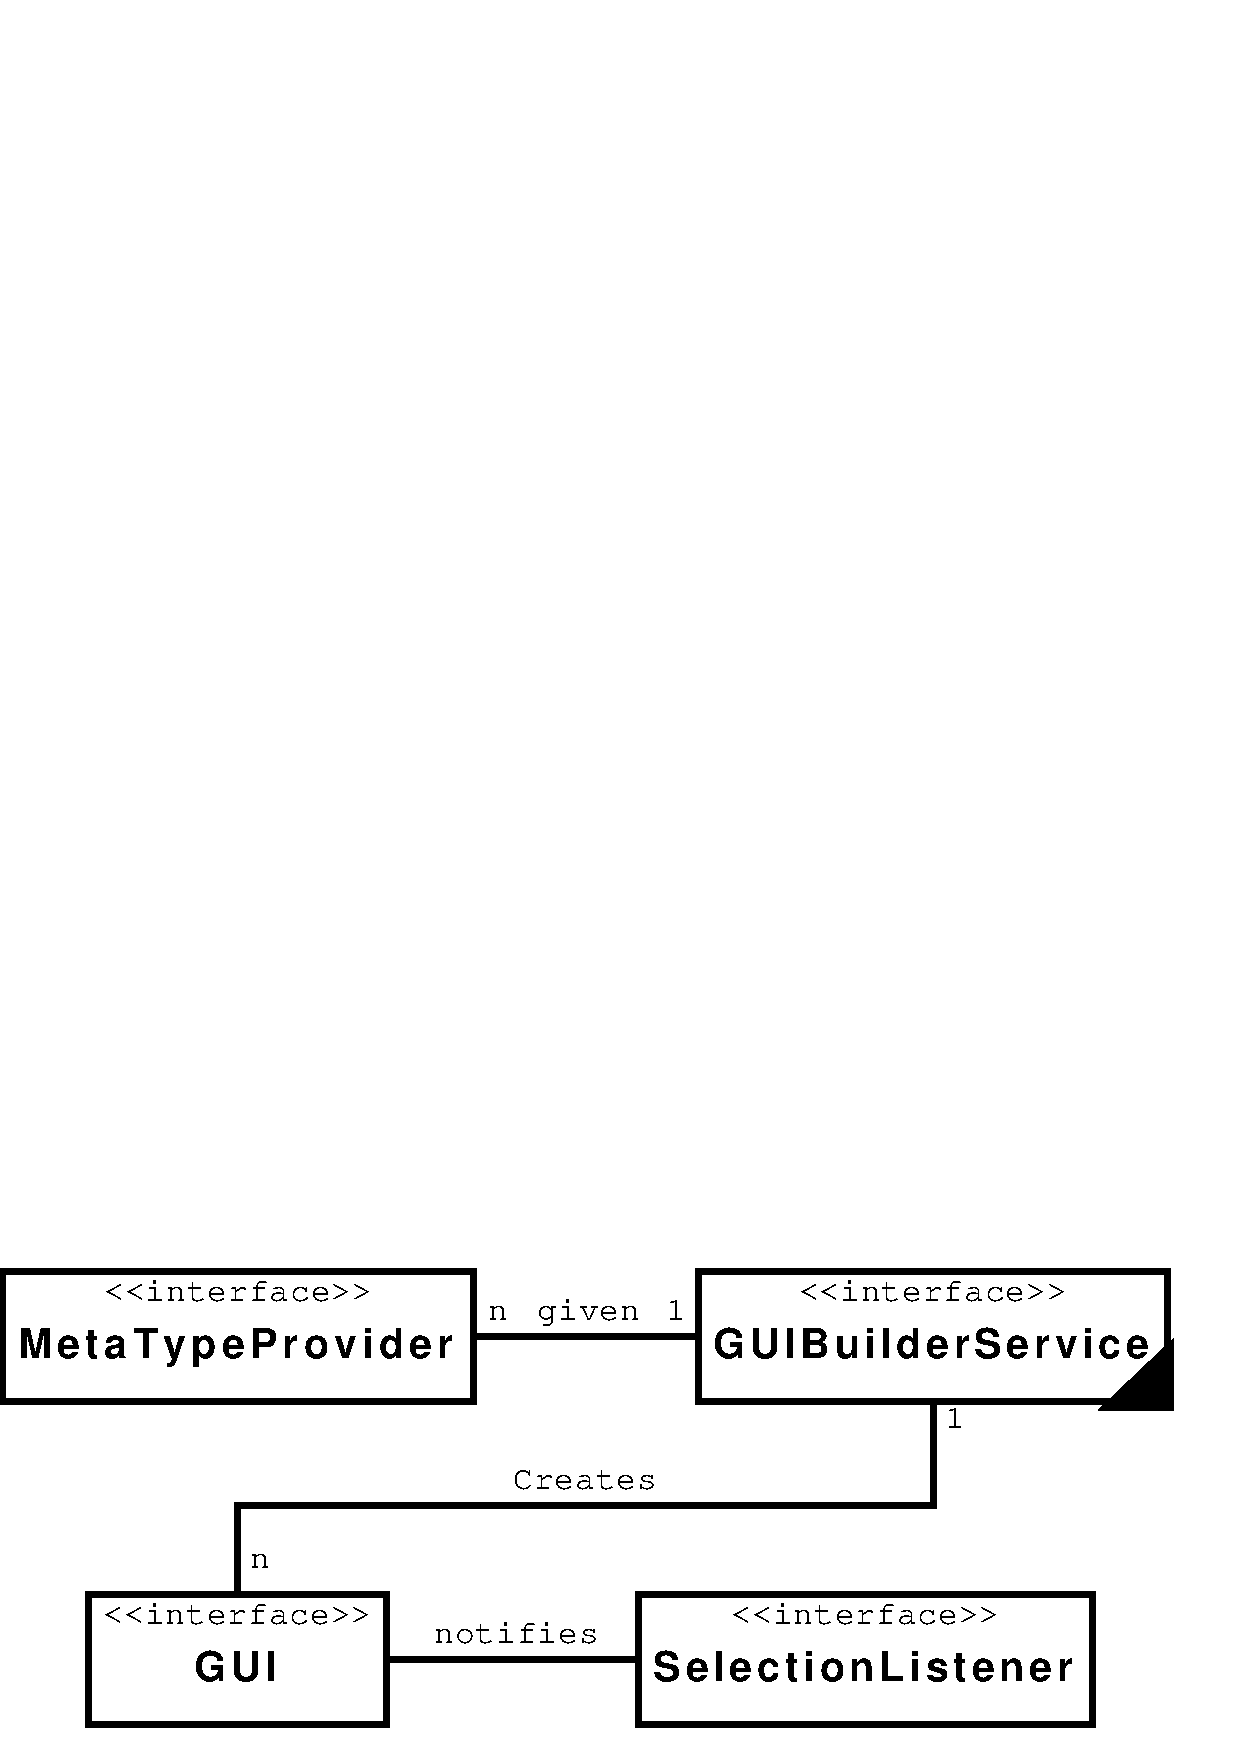
\includegraphics[width=90mm]{../img/guiCreationWorkflow.pdf}
\caption{GUI Creation Workflow}
\label{fig:guiCreationWorkflow}
\end{figure}

\orgcishellserviceguibuilder{}

%% Cyberinfrastructure Shell (CIShell) Core Specification
%%
%% Copyright 2006,2007,2008 Indiana University
%%
%% Licensed under the Apache License, Version 2.0 (the "License");
%% you may not use this file except in compliance with the License.
%% You may obtain a copy of the License at
%%
%%     http://www.apache.org/licenses/LICENSE-2.0
%%
%% Unless required by applicable law or agreed to in writing, software
%% distributed under the License is distributed on an "AS IS" BASIS,
%% WITHOUT WARRANTIES OR CONDITIONS OF ANY KIND, either express or implied.
%% See the License for the specific language governing permissions and
%% limitations under the License.
%%
%

\chapter{Log Service Specification}
\label{logService}
\section*{Version 1.3}
\section{Introduction}

CIShell requires OSGi's standard \class{LogService} to be installed in a
CIShell-compliant system. This gives both the algorithms and the applications
built on CIShell a standard logging sytem to use. This service has not been
extended or modified. More information about the \class{LogService} is available
in the OSGi Service Platform Service Compendium Specification R4, section 101
under ``Log Service Specification.'' Recommended output per log level for
CIShell algorithms are listed in table \ref{table:logLevels}.

\begin{table}[htb!]
\begin{center}
\begin{tabular}{l p{12cm}}
\textbf{Log Level} & \textbf{Recommended Use} \\
LOG\_DEBUG & Used for problem determination and may be irrelevent to anyone but
the algorithm developer. \\
LOG\_ERROR & Indicates a problem occurred while the algorithm was executing.
Indicators of possible fixes should be output to this level along with
relevent information describing what went wrong, if possible. \\
LOG\_INFO & Used for providing information about and while the algorithm is
executing. It does not indicate a problem. \\
LOG\_WARNING & Indicates that the algorithm will still be executed, but
that outputs may not be what was expected. This is often in response to
illogical, but still valid user inputs.
\end{tabular}
\end{center}
\caption{Log Level Recommendations for Algorithms}
\label{table:logLevels}
\end{table}
\chapter{Preferences Service Specification}
\label{preferencesService}
\section*{Version 1.1}
\section{Introduction}

CIShell requires OSGi's standard \class{PreferencesService} to be installed in a
CIShell-compliant system. This gives both the algorithms and the applications
built on CIShell a standard preferences storage system to use. It is used mainly
as a storage mechanism for data that is not necessarily adjustable by end-users.
Things like, last opened file, recently opened files, or any sort of data that
may need to be saved between sessions. This service has not been modified or
extended. More information about the \class{PreferencesService} is available in
the OSGi Service Platform Service Compendium Specification R4, section 106 under
``Preferences Service Specification.'' Algorithm developers wishing to expose
user-adjustable preferences, should refer to section \ref{userPrefsSpec} for
more information on this separate task.

\chapter{Data Manager Application Service Specification}

\section*{\textit{Version 1.0}}

\section{Introduction}

The Data Manager Service is an optional service designed for application
developers to have a central \class{Data} management system. Algorithm
developers may use this too if they wish, but it is not guaranteed to be
available accross all CIShell-compliant systems.

\subsection{Entities}

\begin{itemize}
  \item \textit{DataManagerService} - The service interface for \class{Data}
  management.
  \item \textit{DataManagerListener} - The interface for listening to events
  generated by the \class{DataManagerService}.
  \item \textit{DataManagerAdapter} - This abstract class is an adapter
  implementation of \class{DataManagerListener} with empty method
  implementations.
  \item \textit{Data} - The interface used to pass data (other than
  parameters) and meta-data between algorithms.
\end{itemize}

\section{Data Manager Service}

\comments{Needs to be expanded\ldots}
\comments{Refactor listeners to be services a la:
http://www.osgi.org/documents/osgi\_technology/whiteboard.pdf }

\orgcishellappservicedatamanager{}
%% Cyberinfrastructure Shell (CIShell) Core Specification
%%
%% Copyright 2006,2007,2008 Indiana University
%%
%% Licensed under the Apache License, Version 2.0 (the "License");
%% you may not use this file except in compliance with the License.
%% You may obtain a copy of the License at
%%
%%     http://www.apache.org/licenses/LICENSE-2.0
%%
%% Unless required by applicable law or agreed to in writing, software
%% distributed under the License is distributed on an "AS IS" BASIS,
%% WITHOUT WARRANTIES OR CONDITIONS OF ANY KIND, either express or implied.
%% See the License for the specific language governing permissions and
%% limitations under the License.
%%
%

\chapter{Scheduler Application Service Specification}

\section*{Version 1.0}

\section{Introduction}

The Scheduler Service is an optional service designed for application developers
to schedule algorithms for later monitoring and execution. Algorithm developers
may use this too if they wish, but it is not guaranteed to be available across
all CIShell-compliant systems.

\subsection{Entities}

\begin{itemize}
  \item \textit{SchedulerService} - The service interface for scheduling
  algorithms to be monitored and executed.
  \item \textit{SchedulerListener} - The interface for listening to events
  generated by the \class{SchedulerService}.
  \item \textit{SchedulerAdapter} - This abstract class is an adapter
  implementation of \class{SchedulerListener} with empty method
  implementations.
\end{itemize}

\orgcishellappservicescheduler{}


%%% We have no references thus far, so this is commented out for now. 
% Bibliography:
% \clearpage
% \bibliographystyle{plain}
% \bibliography{../bibliography}

\end{document}
